% interactcadsample.tex
% v1.03 - April 2017

\documentclass[]{interact}

\usepackage{epstopdf}% To incorporate .eps illustrations using PDFLaTeX, etc.
\usepackage{subfigure}% Support for small, `sub' figures and tables
%\usepackage[nolists,tablesfirst]{endfloat}% To `separate' figures and tables from text if required

\usepackage{anyfontsize}% allow to choose any font size in section
\usepackage{natbib}% Citation support using natbib.sty
\usepackage{booktabs} % For prettier tables
\usepackage{graphicx} % For prettier tables
\usepackage{caption,booktabs} % For prettier tables (center the label)

\usepackage{graphicx} % insert figure
\graphicspath{ {./figures/} }

\captionsetup{justification = centering}
\usepackage{hyperref} % linke table to text

\usepackage{har2nat} % Allows to use harvard package with natbib https://mirror.reismil.ch/CTAN/macros/latex/contrib/har2nat/har2nat.pdf

% For citing with natbib, you may want to use this reference sheet: 
% http://merkel.texture.rocks/Latex/natbib.php

\usepackage{setspace}

\usepackage{pdfpages} % we can include pdf figures into the article

\usepackage{algorithm} % for algorithm box
\usepackage{algorithmicx} % for algorithm box
\usepackage{algpseudocode} % for algorithm box

\usepackage{colortbl} % for color table

\theoremstyle{plain}% Theorem-like structures provided by amsthm.sty

\newtheorem{theorem}{Theorem}[section]
\newtheorem{lemma}[theorem]{Lemma}
\newtheorem{corollary}[theorem]{Corollary}
\newtheorem{proposition}[theorem]{Proposition}

\theoremstyle{definition}
\newtheorem{definition}[theorem]{Definition}
\newtheorem{example}[theorem]{Example}

\theoremstyle{remark}
\newtheorem{remark}{Remark}
\newtheorem{notation}{Notation}

\begin{document}
	
	\begin{titlepage}
		\begin{center}
			\vspace*{1.1cm}
			
			\Huge
			\textbf{Changepoint Detection in Social Networks: an Extension of the Relational Event Model}
			
			\vspace{1.8cm}
			\LARGE
			RESEARCH REPORT
			
			\vspace{1.8cm}
			
			\textbf{Hsuan Lee (9252568)}
			
			\vspace{1cm}
			Supervisors: 
			
			\vspace{0.5cm}
			
			Dr. Mahdi Shafiee Kamalabad 
			
			\& 
			
			Dr. Javier Garcia Bernardo
			
			\vspace{2cm}
			\Large
			
			\ Programme: MSBBSS
			
			\vspace{0.3cm}
			
			\emph{Department of Methodology \& Statistics}\\
			
			\vspace{0.3cm}
			Utrecht University\\
			the Netherlands\\
			
			\vspace{1.5cm}    
			\Large
			Date: 08.05.2023
			
			Candidate Journal: Social Networks
			
			FETC Case Number: 22-1870; 22-1871
		
		\end{center}
	\end{titlepage}
	
	\articletype{THESIS PROPOSAL}
	
	\vspace*{1cm}
	\hspace{-0.45cm}{\Large \textbf{Abstract}} \\
	
	Time-stamped relationships dominate our lives, shaping the dynamic nature of our daily interactions with others. From scheduled meetings to social media interactions, the ebb and flow of our daily routines are dictated by time and the people around us. When studying social networks, the Relational Event Model (REM) is a mature model that explains the dynamic nature of these networks. However, it does not inform us when the changepoint of the social network occurs. Understanding the changepoint of a social network can be important, as it allows us to identify the key moments when the network structure underwent significant changes, which can help us better understand the evolution of the network and the underlying social dynamics at play. In this study, we propose a changepoint detection approach under the Relational Event Model (REM) structure. We employ a moving window to segment the event history into windows and fit the REM on each window. We then utilize three state-of-the-art changepoint detection algorithms: Bayesian Online Changepoint Detection (BOCPD), Pruned Exact Linear Time (PELT), and Binary Segmentation (BS), to detect changepoints across windows and compare their performances. Our analysis of synthetic data indicates that BOCPD performs well in terms of precision, as most of the changepoint windows it indicates are highly convincing to be true changepoint windows. PELT is capable of revealing most of the changepoint windows in the network, but this comes at a trade-off with its high number of false positives. BS is the least effective algorithm, as it cannot reveal as many true changepoint windows as PELT and also lacks the high precision of BOCPD. We validate our approach using Apollo 13 voice loop data, which confirms its effectiveness in real-life analysis. The results from the synthetic analysis are consistent with the real-life data, as BOCPD and PELT capture all the potential changepoints that we hypothesize, while BS missing a few. \\
	
	\hspace{-0.45cm}{\textbf{Keywords: }} \\
	{\small{Social network, Relational Event Model, Moving Window approach, Changepoints detection, Binary Segmentation, Pruned Exact Linear Time, Bayesian Online Changepoint Detection Method}
	
	\newpage


	\section{\fontsize{14}{15}\selectfont Introduction}
	
	\hspace{0.2cm} The relational event model (REM) is a mature model for studying real-time social interactions and predicting future events in a social network. It uses factors (e.g., gender, age, interaction inertia, etc.) that shape social interactions, known as ``effects,''\cite{buttsRelationalEventFramework2008} to parameterize the interaction rates between actors. The REM assumes that these effects are constant over time. However, given the dynamic nature of social networks, the strengths of these effects can change over time. Identifying changepoints in the REM can help us understand when social network dynamics change qualitatively. For example, in a classroom setting, students may form social networks based on interests and hobbies that change over time. Identifying these changepoints can help teachers and administrators better support student engagement and social connections, ultimately leading to a more positive learning environment. \\
	
	Changepoints represent sudden shifts in time series data that reflect transitions occurring across conditions\cite{sharmaTrendAnalysisChange2016}\cite{aminikhanghahiSurveyMethodsTime2017}. Changepoint detection is essential in many domains and has been the focus of numerous studies. For example, Rauhameri and Salminen compared the performance of changepoint detection algorithms on IMS data from a portable ion mobility spectrometer\cite{rauhameriComparisonOnlineMethods2022}. Jarušková utilized a maximum type statistics to detect changepoints in hydrological and meteorological series\cite{jaruskovaProblemsApplicationChangePoint1997}. van den Burg and Williams evaluated and compared the performance of changepoint detection algorithms in general situations using 37 real-world time series data from diverse application domains\cite{burgEvaluationChangePoint2022}. In the social network area, Shafiee Kamalabad and Leenders suggested using Bayes Factor to infer changepoints in the REM\cite{shafieekamalabadWhatPointChange2023}. This approach uses the support of two hypotheses from the data to prove the existence of changepoints. However, there have been few studies on changepoint detection under the REM framework apart from this study. \\
	
	The purpose of this study is to propose an approach that facilitates the identification of changepoints in the REM framework. This approach seeks to address the current gap in REM's ability to detect changes in network dynamics. To achieve this, we utilize the moving window approach developed by Mulder and Leenders \cite{mulderModelingEvolutionInteraction2019} in combination with REM, which we refer to as MW-REM. The MW-REM mechanism involves delineating a specific duration of time (i.e., a window) that partially overlaps with the subsequent window. This window then slides over the entire event history, allowing us to observe fluctuations in the effects over time. To detect changepoints in the social network, our method utilizes the effect fluctuations along the windows as input for the changepoint detection algorithms: Binary Segmentation (BS), Pruned Exact Linear Time (PELT), and Bayesian Online Changepoint Detection (BOCPD). These algorithms were identified as top performers in a comparison conducted by van den Burg and Williams \cite{burgEvaluationChangePoint2022} in a general application. \\
	
	In this study, we specifically investigate (1) the effectiveness of our proposed changepoint detection approach under the REM structure, and (2) compare the performances of the three algorithms under our proposed method. To evaluate their feasibility and performance in the context of social network scenarios within MW-REM, we employ synthetic data to calculate metrics such as Confusion Matrix, Mean Squared Error (MSE), and Mean Signed Difference (MSD). We also apply these methods to real-life data to test their external validity. Our method is applicable to any social network scenario, including communication in surgical rooms, interactions between teachers and students, as well as cooperation and competition between companies. The detection of changepoints can facilitate a better understanding of social dynamics, identify potential challenges as they arise, and inform future strategies based on data. The blueprint of our study is depicted in \autoref{Figure 1}. \\
	
    The structure of the paper is as follows: In the next section, the methodology part, we first introduce REM and MW-REM. Next, we introduce the three changepoint detection algorithms we utilized in our study. Then, we discuss how our proposed approach works based on MW-REM and demonstrate how we simulate synthetic data and calculate metrics for comparing the algorithms. Finally, we introduce how we model real-life data, specifically the Apollo 13 voice loop data. In Section 3, the results and discussion part, we present the effectiveness of our method and comparison results between the three changepoint algorithms on synthetic data and real-life data. \\

    \begin{figure}[h]
    	\captionsetup{justification=raggedright}
    	\captionsetup{labelfont={bf}, labelsep=space, font={footnotesize}}
    	\renewcommand{\figurename}{Figure}
    	\centering
    	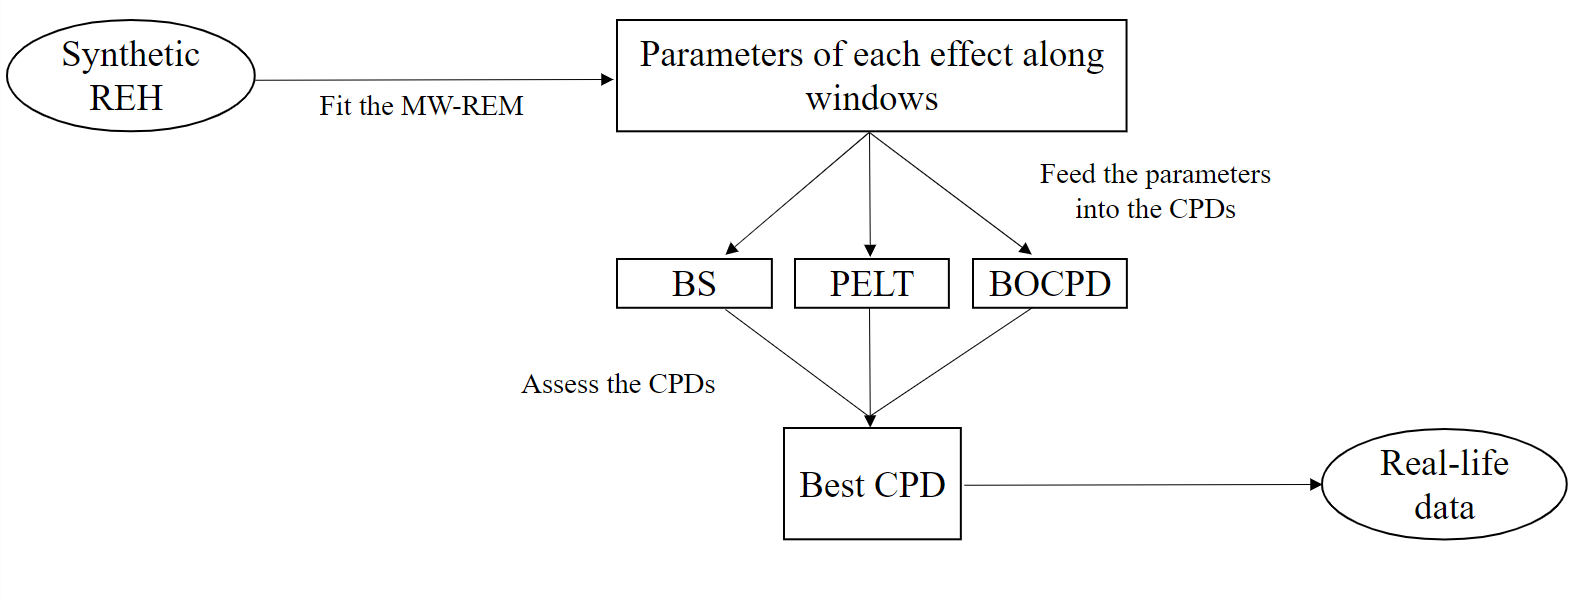
\includegraphics[width=11cm]{Flow_whole}
    	\caption{\fontsize{8}{10}\selectfont Flowchart Depicting the Research Design of the Present Study}
    	\label{Figure 1}
    \end{figure}
	
	\section{\fontsize{14}{15}\selectfont Methodology}
	
	\subsection{Relational Event Model (REM)}
	
	\hspace{0.28cm} The REM is a powerful tool for modeling Relational Event History Data (REH), which at minimum involves sender, receiver, and time information, as shown in \autoref{Table 1}. By analyzing the impact of various effects on the social network, the REM enables us to understand the social interaction dynamic and forecast the timing and participants of the future events in the network. This approach parameterizes both exogenous effects, which are actor characteristics that do not depend on past interactions in the network, such as age or gender, and endogenous effects, which depend on past interactions in the network, such as transitivity or inertia. \\
	
	\begin{table}[h]
		\captionsetup{labelfont={bf}, labelsep=space, font={footnotesize}}
		\centering
		\renewcommand{\arraystretch}{1.1} % increase cell height by 50%
		\small
		\begin{tabular}{llll}
			\hline
			Time (hh,  mm, ss) & sender & receiver & message                                  \\ \hline
			13:14:05           & Patel  & Chen     & The weather conditions look good.        \\
			13:14:09           & Chen   & Patel    & Yes, it should be a smooth flight.       \\
			13:14:12           & Nguyen & Chen     & I've done my safety checks.              \\
			13:14:14           & Chen   & Nguyen   & Great job!                               \\ \hline
		\end{tabular}
		\caption{An Example of Relational Event History Data}
		\label{Table 1}
	\end{table}
	
	To predict the next event in the network, the REM considers every possible sender-receiver combination $(s,r)$ as a potential occurrence at time $t$, and the collection of these pairs at time $t$ is named the risk set, denoted as $R(t)$. The risk set's size for each event is usually $N \times (N-1)$, where $N$ refers to the number of actors in the social network, as each actor can only be either a sender or a receiver, but not both. The REM models the event rate ($\lambda$) for each sender-receiver pair $(s,r)$ to predict which pair will be involved in the next event and when it will occur. The event rate is assumed to remain constant between the time of the present event and the time of the following event, the pair with a higher event rate in the risk set $R$ at time $t$ is more likely to occur in the next event. The probability of the $(s,r)$ pair taking place in the next event follows a multinomial distribution, given by
	\begin{equation} \label{1}
		P \left((s,r) | t \right) = \dfrac{\lambda(s,r,t)} {\sum_{R(t)} \lambda(s,r,t)},
	\end{equation}
	where $\lambda(s,r,t)$ represents the event rate of a pair $(s,r)$ and $R(t)$ denotes the risk set for time $t$. \\
	
	The duration between two events follows an exponential distribution, which is given by
	\begin{equation} \label{2}
		\Delta t \sim Exponential \left(\sum_{R(t)} \lambda(s,r,t) \right),
	\end{equation}
	where $\Delta t$ denotes the duration between two events. The higher the total event rate of the risk set, the shorter the $\Delta t$. \\
	
	The event rate is typically considered as a log-linear function of the outcome in REM with specific effects, given by
	\begin{equation} \label{3}
		\log \lambda(s,r,t) = \sum_{p} \beta_p x_p(s,r,t),
	\end{equation}
	where $\beta_p$ represents the parameter of effects, which expresses the strength of one effect on the entire social network, and $x_p(s,r,t)$ denotes the statistics, which can be either an exogenous or endogenous effects. \\
	
	Despite the REM's outstanding capability in capturing social network dynamics and forecasting, its weakness lies in the assumption that the strength of all effects (i.e., $\beta_p$) remains constant throughout the entire event history. This assumption is unrealistic considering the dynamic property of social interactions. For instance, consider a social network where age is the exogenous effect, and transitivity (i.e., the tendency of friends to have common friends) is the endogenous effect. Initially, age may strongly influence the event rate, indicating that older individuals are more likely to interact. However, this effect may weaken or even reverse over time due to changes in the network's dynamics or cultural norms. Similarly, the strength of the transitivity effect may vary as new friendships form or old ones dissolve. Therefore, assuming that effect strengths remain constant throughout the event history can result in inaccurate predictions and an incomplete understanding of social network dynamics.
	
	\subsection{Moving Window-Relational Event Model (MW-REM)}
	
	\hspace{0.23cm} The Moving Window approach (MW) \cite{mulderModelingEvolutionInteraction2019} addresses the limitations of the REM. The MW involves setting up a fixed-size window, i.e., a fixed length of time, that slides over the entire Relational Event History (REH) data. Each window overlaps with the previous window, and the REM is fitted to each window (see \autoref{Figure 2}). We refer to this approach as MW-REM in this study. The MW-REM allows us to reveal the dynamics of each effect on the social network over time through the effect parameters ($\beta_p$) given in each window. It enables us to investigate the dynamic changes of the effect strengths in social networks over time, a feature not available in the original REM. \\

    \begin{figure}[h]
    	\captionsetup{justification=raggedright}
    	\captionsetup{labelfont={bf}, labelsep=space, font={footnotesize}}
    	\renewcommand{\figurename}{Figure}
    	\centering
    	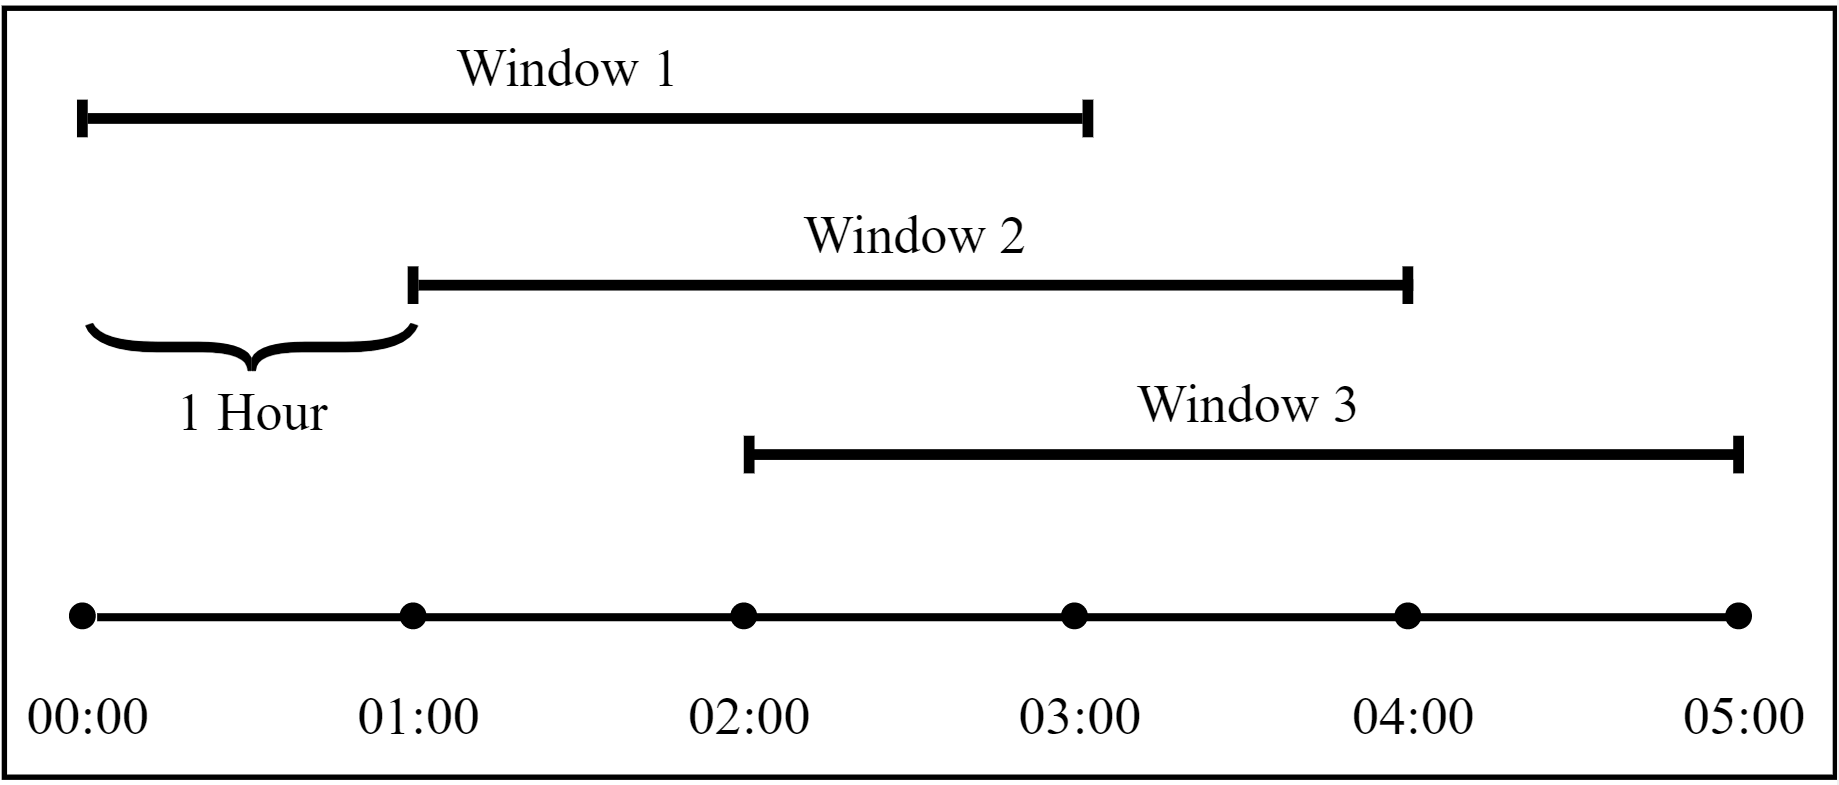
\includegraphics[width=13cm]{MW}
    	\caption{\fontsize{8}{10}\selectfont Example of Moving Window Approach: a window length of 1 hour with an overlap of $\frac{1}{3}$.}
    	\label{Figure 2}
    \end{figure}
    
	% add curly bracket for the plot
	%\begin{picture}(0,0)
	%	\put(36,70.5){\makebox(137.5,4){\upbracefill}}
	%	\put(128.2,104.3){\makebox(137,4){\upbracefill}}
	%	\put(220.3,138){\makebox(137,4){\upbracefill}}
	%\put(100.8,99){\makebox(137,4){\upbracefill}}
	%\end{picture}
	
	\subsection{Changepoint detection}
	
	\hspace{0.2cm} In this study, we propose an approach for detecting changepoints in REH, building on the foundation of MW-REM. As MW-REM divides the event history into partially overlapping sub-portions to fit the REM, it provides us with effect parameters ($\beta_p$) for each window over time, indicating the strength of each effect during that period, as shown in \autoref{3}. By fitting MW-REM to the event history, we obtain as many REMs as the fitting windows, and therefore the same number of effect parameters ($\beta_p$) as the number of fitting windows. \\
	
	Our proposed approach utilizes three changepoint detection algorithms for detecting changepoints in social networks: Binary Segmentation (BS), Pruned Exact Linear Time (PELT), and Bayesian Online Changepoint Detection (BOCPD). According to van den Burg and Williams\cite{burgEvaluationChangePoint2022}, these three changepoint detection algorithms were identified as top performers in a comparison in a general application. The comparison was based on criteria such as $F1$ scores and Segmentation covering metric. We chose these changepoint detection algorithms for their respective advantages and suitability for detecting changepoints in social networks, which can have abrupt changes over time. It is worth noting that changepoint detection algorithms can be classified into two categories, online and offline methods. Online methods aim to detect changes immediately in a real-time context, while offline methods examine changes retrospectively upon collection of complete data \cite{kendrickChangePointDetection2018}. In our study, BS is an offline method, PELT and BOCPD are online methods. The fundamental mechanisms of the three changepoint detection algorithm are presented in the following sections.
	
	\subsubsection{Binary Segmentation (BS)}
	
	%\hspace{-0.55cm} \textbf{Binary Segmentation (BS)}\\
	
	\hspace{0.28cm} Binary Segmentation is a commonly used algorithm for detecting changepoints in time series data. The algorithm is based on a divide-and-conquer approach, which involves recursively splitting the time series into smaller segments until a segment is found that appears to be homogeneous with respect to a statistical property of interest, such as the mean or variance. Once a segment is found to be homogeneous, a changepoint is detected at the boundary between that segment and the previous one\cite{killickOptimalDetectionChangepoints2012}. \\
	
	The key idea behind Binary Segmentation is to minimize a cost function that penalizes the number of changepoints and the size of the segments. The cost function can be thought of as a trade-off between model complexity and goodness of fit. A more complex model with more changepoints may fit the data better, but it will also be more likely to overfit and capture noise in the data. On the other hand, a simpler model with fewer changepoints may underfit and miss important changes in the data. The most common cost function for multiple changepoint detection is given by
	\begin{equation} \label{4}
		\sum_{i = 1} ^{m + 1} \left[C(y_{({\tau_{i-1} + 1}):\tau_{i}}) \right] + \beta f(m),
	\end{equation}
	where $i$ denotes the order of a time point in a segment, $m$ indicates the number of changepoints, $\tau_i$ implies the location of a possible changepoint (i.e., time point $i$). And the m changepoints will divide the data into $m+1$ segments, with the $i$th segment contains $y_{({\tau_{i-1} + 1}):\tau_{i}}$. $C$ represents the cost function of a segment, $\beta f(m)$ serves as a penalty to prevent overfitting\cite{killickOptimalDetectionChangepoints2012}. \\
	
	To trade-off between accuracy and simplicity, BS starts with a single segment that spans the entire time series and recursively splits the segment into two smaller segments at the point that minimizes the cost function. This process continues until no further splits are possible, given by
	\begin{equation} \label{5}
		C(y_{1:\tau}) + C(y_{({\tau + 1}):n}) + \beta < C(y_{1:n}),
	\end{equation}
	In other words, BS searches for possible changepoints until there is no $\tau$ that meets the criteria. At this point, BS stops. Finally, the set of changepoints detected in each segment are merged to obtain the final set of changepoints.
	
	\subsubsection{Pruned Exact Linear Time (PELT)}
	
	%\hspace{-0.55cm} \textbf{Pruned Exact Linear Time (PELT)}\\
	
	\hspace{0.23cm} PELT is another algorithm for detecting changepoints in time series data. Like Binary Segmentation, PELT is a divide-and-conquer approach that recursively splits the time series into smaller segments. However, PELT differs from Binary Segmentation in that it has a computational complexity that is linear with respect to the length of the time series\cite{killickOptimalDetectionChangepoints2012}, making it more efficient. \\
	
	The key idea behind PELT is to iteratively remove candidate changepoints that do not significantly reduce the cost function in \autoref{4}. Specifically, PELT starts with a single segment that spans the entire time series, and then recursively splits the segment into smaller segments at the point that minimizes the cost function\cite{chapmanMetaAnalysisMetricsChange}. At each step, PELT evaluates the cost of adding a new changepoint between each pair of adjacent segments. If the cost of adding a new changepoint is not significant, the algorithm prunes the candidate changepoint and continues with the next pair of adjacent segments. This process is repeated until no further candidate changepoints remain. \\
	
	The final set of changepoints detected by PELT is obtained by merging the remaining candidate changepoints with the ones detected in each smaller segment. The resulting set of changepoints provides an exact solution that minimizes the cost function in \autoref{4} with the fewest possible number of changepoints.
	
	\subsubsection{Bayesian Online Changepoint Detection (BOCPD)}
	
	%\hspace{-0.55cm} \textbf{Bayesian Online Changepoint Detection (BOCPD)}\\
	
	\hspace{0.27cm} Unlike the BS and PELT, which rely on cost functions to identify changepoints, Bayesian Online Changepoint Detection (BOCPD) infers changepoints based on a Bayesian approach, which defines changepoints in terms of posterior probabilities, also known as run length probabilities, at time points. \\
	
	In BOCPD, run length is an essential concept, representing the length of time elapsed since the last identified changepoint. This can be understood as akin to the segments in PELT and BS. Whenever BOCPD recognizes a changepoint, the run length drops to 0 and recalculates the length. To determine the changepoints, BOCPD calculates the run length probabilities (i.e., posterior probabilities) for each time point, which include both growth probabilities and changepoint probabilities. \\
	
	According to Adams and Mackay\cite{adamsBayesianOnlineChangepoint2007}, to save computational costs, it is suggested to set a cut-off point for the run length probability, typically $10^{-4}$. If the run length probability reaches such a cut-off point, the time point is determined as a changepoint. \\
	
	Overall, BOCPD starts by building the predictive distribution from the potential locations of changepoints, which reveals any prior knowledge regarding the data generation process. Based on the given predictive distribution, BOCPD computes the run length probability at a time point. As new data come in, the predictive distribution is continuously updated, and BOCPD iteratively runs the same procedure until no new data appear.
	
	\subsubsection{MW-REM Based Changepoint Detection}
	
	\hspace{0.27cm} In this section, we describe the settings used for each of the three changepoint detection methods employed in our paper, as well as our proposed approach based on the MW-REM structure. \\
	
	Dehling and Fried et al. have noted that the mean difference, a commonly used statistical interest in changepoint detection, is not robust to outlying observations in time series\cite{dehlingRobustMethodShift2020}. The mean difference only looks for changes in the mean value, assuming a constant variance. Similarly, variance difference looks for changes in the variance only, assuming a constant mean. To improve changepoint identification, in our study using BS and PELT, we take changes in both the mean and variance into account. In contrast, BOCPD does not rely on statistical interest such as mean or variance to identify changepoints. Instead, it uses a cut-off point for the run length probability. In this study, we follow Adams and Mackay's suggestion to set a cut-off point at $10^{-4}$\cite{adamsBayesianOnlineChangepoint2007}. \\
	
	Algorithm \ref{Algorithm1} shows the details and steps of our proposed five-step approach for identifying changepoints in social networks.
	
	\begin{algorithm}[H]
		\caption{MW-REM Based Changepoint Detection}\label{Algorithm1}
		\begin{algorithmic}[1]
			\State \textbf{Input:} A relational event history (REH) dataset.
			\State Select the effects that drive social interactions using prior knowledge, statistical tests, or other methods.
			\State Select an appropriate window length and overlap (e.g., 2000 seconds with $\frac{2}{3}$ overlap).
			\State Fit the Moving Window Relational Event Model (MW-REM) to the REH dataset.
			\State Extract the parameters ($\beta_p$) of each effect from each window's REM: $\log \lambda(s,r,t) = \sum_{p} \beta_p x_p(s,r,t)$.
			\State Apply Bayesian, frequentist, or other changepoint detection methods to each effect's parameters to identify potential windows that may contain changepoints.
			\State \textbf{Output:} Potential changepoint windows for each effect in the social network.
		\end{algorithmic}
	\end{algorithm}

	\subsection{Generation of synthetic REH data}
	
	\hspace{0.2cm} To evaluate the effectiveness of our proposed changepoint detection approach for REH data, we generated synthetic datasets with various changepoint settings. For each setting, we created 15 datasets that were simulated based on the REH characteristics. These synthetic datasets were constructed using a social network consisting of 30 actors and 10,000 events.\\
	
	To construct these datasets, we randomly selected two exogenous effects and two endogenous effects. We then specified the parameter values ($\beta_p$) for each effect and its changes over time. The assignment of the effects' parameters in the synthetic data is based on Meijerink-Bosman's study\cite{meijerink-bosmanDiscoveringTrendsSocial2022} with slight adjustments. The exogenous effects include the "Sender effect," which represents the actor's exogenous attributes that impact their event sending rate, and the "Difference effect," which indicates the difference in personal attributes that influence the rate of sending events. The endogenous effects consist of the "Inertia effect," which describes the tendency of actors to repeatedly select the same receiver for their events, and the "Outdegree of the Sender effect," which indicates the inclination of actors to send events if they have previously sent more events. 
	The complete parameter assignments can be found in \autoref{Table 2}. \\
	
	Using the assigned parameters of the effects, each sender-receiver pair $(s,r)$ in the risk set $R$ obtained the probability of occurrence at every event, as shown in \autoref{1}. We then built the REH by selecting the $(s,r)$ pair with the highest probability at each event. In this study, we designed five different changepoint settings with varying numbers of changepoints. For each setting, we simulated 15 REH datasets:
	
    \begin{itemize}
    	\item No changepoint:
    	\begin{itemize}
    		\item All of the effects do not have any changepoints. \\
    	\end{itemize}
    	\item One changepoint:
    	\begin{itemize}
    		\item The inertia effect has 1 changepoint, but the rest do not.
    		\item All of the effects have 1 changepoint. \\
    	\end{itemize}
    	\item Two changepoints:
    	\begin{itemize}
    		\item The inertia effect has 2 changepoints, but the rest do not.
    		\item All of the effects have 2 changepoints.
    	\end{itemize}
    \end{itemize}

    For the setting with one changepoint, we set the changepoint for the effect(s) parameter at $t$ = 38200 seconds, which corresponds to the window of 56-58. For the setting with two changepoints, we set the changepoints for the effect(s) parameters at $t$ = 16750 seconds and $t$ = 53900 seconds, corresponding to the windows of 24-26, and 79-81, respectively.

    \begin{table}[H]
    	\captionsetup{justification=raggedright}
    	\captionsetup{labelfont={bf}, labelsep=space, font={footnotesize}}
    	\centering
    	\renewcommand{\arraystretch}{1.15} % increase cell height by 50%
    	\small
    	\begin{tabular}{l|cccc}
    		\hline
    		& \textit{Sender}                                                  & \textit{Difference}                                                & \textit{Inertia}                                                  & \textit{OutdegreeSender}                                          \\ \hline
    		\textit{(1) All have no changepoint}      & 0.1                                                              & -0.1                                                               & 0.18                                                              & 0.12                                                              \\ \hline
    		\textit{(2) Inertia has one changepoint}  & 0.12                                                             & -0.1                                                               & \begin{tabular}[c]{@{}c@{}}0.15 \\ $\to$ 0.06\end{tabular}            & 0.12                                                              \\ \hline
    		\textit{(3) All have one changepoint}     & \begin{tabular}[c]{@{}c@{}}0.18\\ $\to$ 0.04\end{tabular}            & \begin{tabular}[c]{@{}c@{}}-0.05 \\ $\to$ -0.15\end{tabular}           & \begin{tabular}[c]{@{}c@{}}0.13 \\ $\to$ 0.06\end{tabular}            & \begin{tabular}[c]{@{}c@{}}0.13 \\ $\to$ 0.07\end{tabular}            \\ \hline
    		\textit{(4) Inertia has two changepoints} & 0.12                                                             & -0.11                                                              & \begin{tabular}[c]{@{}c@{}}0.01 \\ $\to$ 0.12 \\ $\to$ -0.01\end{tabular} & 0.12                                                              \\ \hline
    		\textit{(5) All have two changepoints}    & \begin{tabular}[c]{@{}c@{}}0.2 \\ $\to$ -0.01 \\ $\to$ 0.19\end{tabular} & \begin{tabular}[c]{@{}c@{}}-0.01 \\ $\to$ -0.12 \\ $\to$ 0.03\end{tabular} & \begin{tabular}[c]{@{}c@{}}0.02 \\ $\to$ 0.14 \\ $\to$ 0.03\end{tabular}  & \begin{tabular}[c]{@{}c@{}}-0.01 \\ $\to$ 0.14 \\ $\to$ 0.01\end{tabular} \\ \hline
    	\end{tabular}
        \caption{The assignment of parameter values for the effects in the synthetic data. The rows represent the different changepoint settings, the columns represent the individual effects. The arrows indicate the parameter values before and after the changepoint.}
        \label{Table 2}
    \end{table}

	\subsection{The evaluations of changepoint detection algorithms}
	
	\hspace{0.28cm} Having generated synthetic REH data with different changepoint settings, we proceeded to evaluate the effectiveness of our proposed changepoint detection approach on these datasets. To this end, we fitted the MW-REM with a window length of 2000 seconds and $\frac{2}{3}$ overlap to each dataset and extracted the effects' parameters. In Meijerink-Bosman's 2022 study, a window length of 2000 seconds and $\frac{2}{3}$ overlap were found to be sufficient for capturing the effect dynamics with reasonable accuracy \cite{meijerink-bosmanDynamicRelationalEvent2022}. Although this setting may miss some of the finer network details, it is computationally efficient compared to using smaller window sizes, and the effects fluctuations over time are relatively less noisy. \\
	
	In the following section, we describe how we inspected the performance and compared three changepoint detection algorithms applied to these extracted parameters, utilizing three metrics: the confusion matrix, mean squared error (MSE), and mean signed difference (MSD). %For each metric, we summarize the performance of the changepoint detection algorithms for the following categories: no changepoint, one changepoint, and two changepoints.
	
	\subsubsection{Confusion matrix}
	
	\hspace{0.28cm} After feeding the changepoint detection algorithms with the effects' parameters, we used the confusion matrix to evaluate the performance of each algorithm for each effect. A true positive indicates that the algorithm correctly detected a window containing the changepoint of the effect. Notably, due to the overlapping property of the windows, a changepoint can be contained in three consecutive windows simultaneously. Therefore, if an algorithm detects the changepoint in any of the three windows, it is considered a true positive. However, since the synthetic datasets are produced based on selecting the $(s,r)$ pair with the highest rate probability in the risk set $R$ for every event, the locations of the changepoints may differ slightly from our assignment. As a result, if a changepoint detection algorithm detects a changepoint within the range of three windows of the windows containing the true changepoint, we consider it a true positive. \\
	
	A false positive indicates that the algorithm falsely detected a window as a changepoint, while a false negative indicates that the algorithm failed to detect a window containing the changepoint of the effect. However, our synthetic datasets are highly imbalanced, with many windows and few changepoints, so we did not take the true negative into account. \autoref{Table 2} presents the confusion matrix for changepoint detection, showing the actual and predicted changepoints and non-changepoints. \\
	
	\begin{table}[h]
	\captionsetup{labelfont={bf}, labelsep=space, font={footnotesize}}
	\centering
	\renewcommand{\arraystretch}{1.5} % increase cell height by 50%
	\small
	\begin{tabular}{l|c|c}
		\hline
		& \textit{Actually Changepoint} & \textit{Actually Not Changepoint}                   \\ \hline
		\textit{Predicted Changepoint} & True Positive              & False Positive                               \\ \hline
		\textit{Predicted Not Changepoint} & False Negative             & \multicolumn{1}{l}{\cellcolor[HTML]{C0C0C0}} \\ \hline
	\end{tabular}
	\caption{Confusion Matrix for changepoint detection}
	\label{Table 3}
    \end{table}
	
	Given the information from the confusion matrix, we employ three indicators to assess the effectiveness of our proposed approach and the performance of the three changepoint detection algorithms in detecting changepoints in REH. The first indicator is the number of false positive cases. We separately sum the number of false positives of the effects with no changepoint, one changepoint, and two changepoints for each changepoint detection algorithm. For instance, if the REH has one changepoint in the inertia effect, but not for the other effects, the number of false positives of the inertia effect by a changepoint detection algorithm is summed in the one changepoint group, while the rest of the effects are summed in the no changepoint group. This is done to determine which of the three changepoint algorithms has the highest likelihood of falsely detecting a changepoint when there is none, considering the no changepoint, one changepoint, and two changepoints settings for each effect. \\
	
	The second indicator is the true positive rate (TPR). Similar to the false positives indicator, we separate the effects into groups based on their number of changepoints. However, since there are no true positives for the effects with no changepoint, we only consider the groups with one and two changepoints for each changepoint detection algorithm. The TPR is calculated as follows:
	
	\begin{equation} \label{7}
		TPR_g = \frac{TP_g}{TP_g + FN_g}
	\end{equation}
    , where $TP$ indicates the number of true positive cases, $FN$ indicates the number of false negative cases, and $g$ indicates the changepoint group. Through the TPR, we obtain information about the probability that each changepoint detection algorithm correctly predicts the true positive for the effects with one or two changepoints, respectively, among all positive observations. \\

    The third indicator is the positive predictive value (PPV). Similar to the TPR and false positives indicators, we also group the effects into one changepoint and two changepoint groups based on their number of changepoints. The PPV is calculated as:
 
    \begin{equation} \label{8}
    	PPV_g = \frac{TP_g}{TP_g + FP_g}
    \end{equation}
	, where $TP$ represents the number of true positive cases, $FP$ represents the number of false positive cases, and $g$ represents the changepoint group. The PPV indicates the probability that a predicted changepoint is indeed a changepoint, providing insight into the precision of the changepoint detection algorithms.
	
	\subsubsection{Mean Squared Error (MSE) \& Mean Signed Difference (MSD)}
	
	\hspace{0.28cm} To evaluate the performance of each changepoint detection algorithm, we use mean squared error (MSE) and mean signed difference (MSD) as measures to examine the accuracy of the predicted changepoint window and the tendency of the algorithm to detect changepoints early or late. \\
	
	The MSE measures the average squared distance between the predicted and actual changepoint windows for each changepoint detection algorithm. We compute the MSE only for true positive cases from the confusion matrix of each effect. Specifically, we calculate the MSE as follows \cite{aminikhanghahiSurveyMethodsTime2017}:
	
	\begin{equation} \label{9}
		MSE = \frac{\sum_{i = 1}^{\#CP} (Predicted(CP) - Actual(CP))^2}{\#CP}
	\end{equation}
	,where $CP$ denotes the windows containing a changepoint, and $\#CP$ represents the number of changepoints in the REH. The lower the MSE, the higher the precision of the algorithm. To evaluate the performances of the changepoint detection algorithms across different changepoint scenarios, we group the effects into one-changepoint and two-changepoint groups and report the average MSE of each group for each algorithm using the following formula:
	
	\begin{equation} \label{10}
		Avg.MSE_g = \frac{\sum_{i=1}^{N_g} MSE_i}{N_g}
	\end{equation}
	, where $Avg.MSE_g$ represents the average MSE for group $g$, $MSE_i$ is the MSE value for the $i$th effect in group $g$, and $N_g$ is the number of effects in group $g$. \\
	
	The MSD, on the other hand, is used to examine the tendency of the changepoint detection algorithm to detect changepoints early or late. We compute the MSD only for true positive cases from the confusion matrix of each effect. Specifically, we calculate the MSD as follows:
	
	\begin{equation} \label{11}
		MSD = \frac{\sum_{i = 1}^{\#CP} (Predicted(CP) - Actual(CP))}{\#CP}
	\end{equation}
	, here, a negative MSD indicates that the changepoint detection algorithm tends to predict the changepoint window earlier than the true changepoint window, while a positive MSD indicates that the algorithm tends to predict the changepoint window later than the true changepoint window. \\
	
	To evaluate the changepoint detection algorithms' detection tendencies under different changepoint scenarios, we group the effects into one-changepoint and two-changepoint groups. The average MSD of each group for each algorithm is reported using the following formula:
	
	\begin{equation} \label{12}
		Avg.MSD_g = \frac{\sum_{i=1}^{N_g} MSD_i}{N_g}
	\end{equation}
	, where $Avg.MSD_g$ represents the average MSD for group $g$, $MSD_i$ is the MSD value for the $i$th effect in group $g$, and $N_g$ is the number of effects in group $g$. This allows us to assess each changepoint detection algorithm's tendency to detect changepoints early or late in both univariate and multivariate changepoints scenarios of effects.
	
	\subsection{Manipulation of real-life Apollo 13 voice-loop data}
	
	\hspace{0.2cm} The study utilized real-life data from the publicly available Apollo 13 voice loop data, which captured the communication between the astronauts and Mission Control during the failed Apollo 13 mission. This mission aimed to land on the Moon, but a routine agitation of one of the oxygen tanks caused an explosion that damaged the wire insulation inside, resulting in the discharge of the contents of both oxygen tanks. This left the astronauts without systems to generate electricity and oxygen, prompting them to contact Mission Control for assistance, and ultimately leading to the cancellation of the mission. The analyzed data covers the period from one hour before the emergency until Apollo 13 was safely back on a trajectory towards Earth, specifically from 54:46:28 to 62:06:53 (hh:mm:ss) of the mission timeline. \\
	
	In the Apollo 13 voice loop data, a pivotal moment occurred when an astronaut stated, "I believe we've had a problem here," at 55:55:21. This moment marks the start of the emergency, and we have selected it as the location of the changepoint in our study. We hypothesize that the old interaction patterns were disrupted after this point, making it an ideal location to test the effectiveness of our proposed changepoint detection approach on a real social network. \\
	
	To apply our proposed changepoint detection approach (see Algorithm \autoref{Algorithm 1}), we selected several effects that have a relationship with the network. These effects include the "Inertia effect," which refers to the tendency for actors to repeatedly interact with each other, the "Outdegree of the sender effect," which refers to the tendency for actors to send events if they have sent more past events, the "Indegree of the receiver effect," which refers to the tendency for actors to receive events if they have received more past events, and the "Total degree of the sender effect," which refers to the tendency for actors to send events if they have sent and received more past events. We also selected three other effects that capture specific patterns of interaction: the "AB-BA pshift," which refers to the tendency for immediate reciprocation, where the next sender is the current receiver and the next receiver is the current sender, the "AB-XA pshift," which refers to a tendency for turn usurping, where the next sender is not in the current event and the next receiver is the current sender, and the "AB-BY pshift," which refers to a tendency for turn receiving, where the next sender is the current receiver and the next receiver is not in the current event. \\
	
	Considering the findings of Meijerink-Bosman's research \cite{meijerink-bosmanDynamicRelationalEvent2022}, we decide to fit the MW-REM with a 1000-second window length and $\frac{2}{3}$ overlap, as it provided a good insight into the dynamic of the social network. We then apply this window setting to the Apollo 13 voice loop data, extract the parameters of each effect along the windows, and feed them to the three changepoint detection algorithms employed in our study. \\
	
	In an ideal situation, by feeding the parameters of the effects to the changepoint detection algorithms, they could successfully detect the presence of changepoints for each effect in the MW-REM, around or precisely at the windows that contain the message reporting the issue.
	
	\section{\fontsize{14}{15}\selectfont Results}
	
	\subsection{Synthetic REH datasets analysis}
	
	\hspace{0.28cm} In this section, we present the results of the changepoint detection analysis conducted on the synthetic REH data. As previously described in the methodology section, we summarize the performance of three changepoint detection algorithms applied to the effects' parameters for zero, one, and two changepoints, respectively. We evaluated the algorithms' performance using (1) the number of false positives, (2) true positive rate, (3) positive predictive value, (4) average MSE, and (5) average MSD.
	
	\subsubsection{The number of false positives}
	
	\hspace{0.28cm} As mentioned in the methodology section, a detected changepoint window is considered a true positive if it is within three windows of the true changepoint window. A detected changepoint window is considered a false positive if it is not within the three-window range of the true changepoint window. \\
	
	The synthetic data reveals that, for effects without a changepoint, BOCPD produces a total of 10 false positive cases, while BS and PELT produce 24 and 44 false positives, respectively. For effects with one changepoint, BOCPD generates 5 false positives, while BS and PELT produce 13 and 19 false positives, respectively. For effects with two changepoints, BOCPD results in 2 false positives, while BS and PELT produce 6 and 20 false positives, respectively. Overall, as \autoref{Figure 3} shows, BOCPD performs better than the other algorithms in correctly identifying the window that is not a changepoint window, while PELT is the most prone to incorrectly identifying non-changepoint windows as changepoint windows.
	
	\subsubsection{True positive rate (TPR)}
	
	\hspace{0.28cm} Regarding TPR, \autoref{Figure 3} shows that all three changepoint detection algorithms have similar TPR values when there is a univariate changepoint in the effect, with BOCPD having 0.52, PELT having 0.49, and BS having 0.53. However, in the case of multivariate changepoints, the TPR values significantly improve, with BOCPD having 0.75, PELT having 0.79, and BS having 0.73. It is noteworthy that the improvement in TPR values for all three algorithms is substantial when moving from the univariate to multivariate changepoint situation. This indicates that if an effect has only one changepoint throughout the entire REH, the probability of correctly detecting the window within a range of three windows from the true changepoint window using any of the three algorithms is only around 50\%. On the other hand, if an effect has two changepoints throughout the entire REH, the probability of correctly detecting the window within a range of three windows from the true changepoint window using any of the three algorithms is above 70\%, with PELT almost reaching 80\% in the case of multivariate changepoints. However, PELT's high TPR may be a trade-off with its high false positive cases, as it detects more changepoints, which increases the likelihood of covering more true positives in its prediction.

    \subsubsection{Positive predictive value (PPV)}
    
    \hspace{0.28cm} Moving on to PPV, it measures the proportion of detected changepoints that are true positive changepoints (i.e., within a range of three windows from the true changepoint) out of all detected changepoints. In other words, it evaluates the precision of the changepoint detection algorithms. For effects with one changepoint, BOCPD has the highest PPV, followed by BS and PELT, with BOCPD's positive predictive value being 0.89, while BS and PELT have 0.75 and 0.66, respectively. For effects with two changepoints, BOCPD still has the highest positive predictive value of 0.98, followed by BS with 0.95 and PELT with 0.86. \\
    
    Overall, as shown in \autoref{Figure 3}, there is an improvement in PPV for all three changepoint detection algorithms when moving from the univariate to the multivariate changepoint situation, with all three algorithms having a PPV above 0.85 in the multivariate changepoint situation. This indicates that the probability of a predicted changepoint being within three windows range of the true changepoint is higher than 85\% in the multivariate changepoint situation. Furthermore, BOCPD consistently performs at a high level in terms of PPV, whether in the univariate or multivariate changepoint situation, indicating that the changepoints identified by BOCPD have a high probability of being within three windows range of the true changepoints. Conversely, PELT exhibits the worst performance in terms of PPV, which is influenced by its high false positive rate.
	
	\begin{figure}[h]
		\captionsetup{justification=raggedright}
		\captionsetup{labelfont={bf}, labelsep=space, font={footnotesize}}
		\renewcommand{\figurename}{Figure}
		\centering
		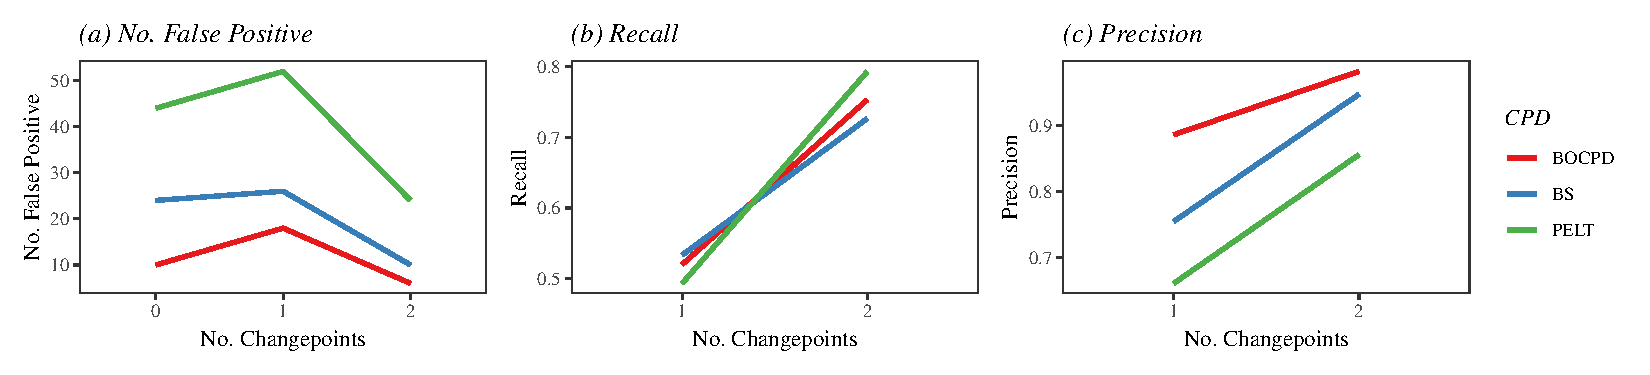
\includegraphics[width=\textwidth,height=\textheight,keepaspectratio]{FPTPRPPV}
		\caption{\fontsize{8}{10}\selectfont The plot shows the number of false positives, true positive rate, and positive predictive value of the three changepoint detection algorithms for effects without changepoint, effects with one changepoint, and effects with two changepoints.}
		\label{Figure 3}
	\end{figure}

    \subsubsection{Average mean squared error (Average MSE)}
    
    \hspace{0.28cm} The average MSE measures the average squared distance between the predicted and actual changepoint windows for different changepoint situations. A lower MSE value indicates greater precision. In the case of a single changepoint, BOCPD has an average MSE of 1.59, while BS and PELT have MSE values of 1.18 and 1.49, respectively. When there are two changepoints, BOCPD has an average MSE of 1.12, BS has an MSE of 0.76, and PELT has an MSE of 0.94. Overall, BS performs the best out of the three algorithms in both univariate and multivariate changepoint situations, indicating that it has the lowest differences between its predicted and actual changepoint windows (see \autoref{Figure 4}). All three algorithms also perform better in the two changepoint situation, suggesting that their predictions of changepoint window location are more reliable in the multivariate changepoint context compared to the univariate changepoint context.

    \subsubsection{Average mean signed difference (Average MSD)}
    
    \hspace{0.28cm} The average MSD provides information about how well a changepoint detection algorithm predicts the location of the changepoint window relative to the true changepoint, for different changepoint situations. A negative value indicates that the algorithm is more likely to predict the window before the true changepoint, while a positive value indicates that it is more likely to predict the window after the true changepoint. \\
    
    In the single changepoint scenario, the BOCPD has an average MSD of 0.05, the BS has -0.03, and PELT has 0.03. In the two changepoint scenario, the BOCPD has an average MSD of 0.12, the BS has -0.1, and PELT has -0.09. From \autoref{Figure 4}, it's clear that the BOCPD tends to detect the changepoint window after the true changepoint, whether in the univariate or multivariate changepoint context. In contrast, the BS tends to detect the window before the true changepoint, and PELT has mixed performance. Interestingly, the reason why BS and PELT tend to detect the changepoint window before the true changepoint is that they are bottom-up methods that merge small intervals based on a cost function balancing data likelihood and model complexity \cite{killickOptimalDetectionChangepoints2012}. This approach favors fewer, larger changepoints and may lead to detecting changepoints slightly before the true location. Additionally, it's possible that the true changepoint window is located in a region of the time series where the effect parameters are already changing but have not yet fully transitioned to the new regime.
    
    \begin{figure}[h]
    	\captionsetup{justification=raggedright}
    	\captionsetup{labelfont={bf}, labelsep=space, font={footnotesize}}
    	\renewcommand{\figurename}{Figure}
    	\centering
    	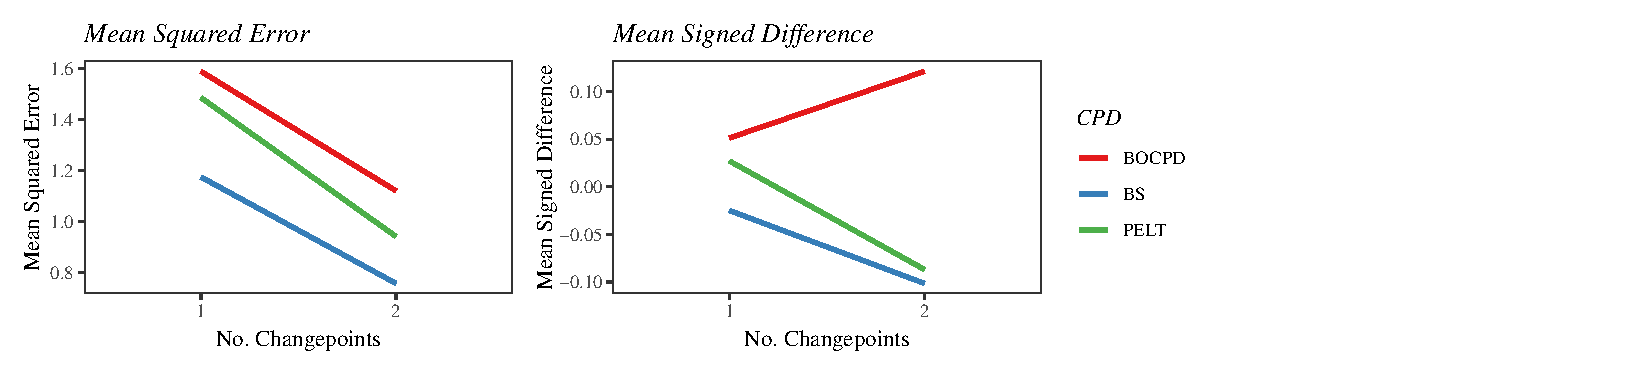
\includegraphics[width=\textwidth,height=\textheight,keepaspectratio]{MSEMSD}
    	\caption{\fontsize{8}{10}\selectfont The plot shows the average mean squared error, and average mean signed difference of the three changepoint detection algorithms for effects with one changepoint, and effects with two changepoints.}
    	\label{Figure 4}
    \end{figure}

    \subsubsection{Conclusion}

    \hspace{0.28cm} The synthetic data analysis confirms the effectiveness of our proposed changepoint detection approach for the MW-REM structure. By feeding the changepoint detection algorithms with the effect parameters given by windows, we can identify the points at which each effect changes in the social network. \\
    
    Regarding the performance of the three changepoint detection algorithms on our method, we can conclude that the BOCPD performs well in terms of PPV, indicating that the changepoints identified by the BOCPD are highly likely to be the true changepoints or within a three-window range of the true changepoint. The PELT has good performance on TPR, indicating that the true changepoints are likely to be covered by all the predicted changepoints from PELT. However, this comes at a cost of high false positives. The BS performs well in terms of MSE, indicating that the location of the predicted changepoint window is close to the true changepoint window.
    
	\subsection{Real-life Apollo 13 data analysis}
	
	\hspace{0.28cm} The emergency report of Apollo 13 occurred at $t$ = 55:55:21 (hh:mm:ss). The MW-REM was applied with a 1000-second window length and $\frac{2}{3}$ overlap, resulting in a total of 76 windows. The actual changepoint window for our study corresponds to the window from 9 to 11, covering the time slot from 55:38:53 to 56:06:40. \autoref{Figure 5} depicts the fluctuations in each effect's parameters over the REH in a single figure. \\
	
    \begin{figure}[h]
    	\captionsetup{justification=raggedright}
    	\captionsetup{labelfont={bf}, labelsep=space, font={footnotesize}}
    	\renewcommand{\figurename}{Figure}
    	\centering
    	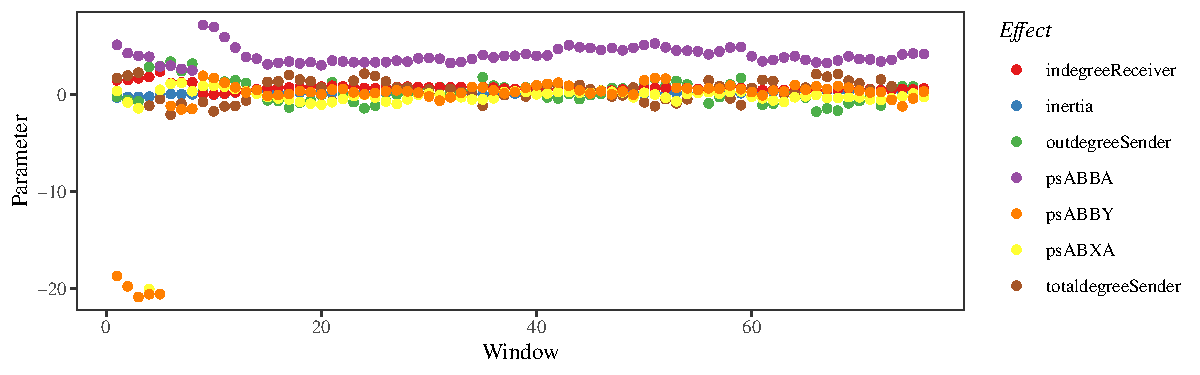
\includegraphics[width=\textwidth,height=\textheight,keepaspectratio]{Apollo_effects}
    	\caption{\fontsize{8}{10}\selectfont The figure shows the wave of effect parameters crossing the 76 windows of each of the seven effects we included in the MW-REM.}
    	\label{Figure 5}
    \end{figure}
	
	We inputted the effect parameters obtained from the MW-REM windows into three different changepoint detection algorithms: BOCPD, BS, and PELT. The resulting changepoint detections are displayed in \autoref{Figure 6}. It is worth noting that the emergency happened between windows 9 and 11, so we anticipated that the algorithms would detect the emergency during or around that timeframe. \\
	
	For the indegree of the receiver effect, BOCPD detected changepoints at windows 9, 15, and 37. BS detected them at windows 6, 8, 12, 15, and 36. PELT detected them at windows 6, 8, 14, 32, and 35. BOCPD successfully captured the changepoint window at 9 and also detected window 15, which occurred four windows later than the actual changepoint window, BS and PELT did not capture any exact window that contained the emergency. BS detected a window that occurred one window before it, and a window that occurred four windows later than it. PELT detected a window that occurred one window ahead of it, and another that was three windows later than it. As we mentioned in the previous section, BS and PELT tend to detect the changepoint window before the true changepoint due to their cost function \cite{killickOptimalDetectionChangepoints2012}, which favors fewer, larger changepoints and may lead to detecting changepoints slightly before the true location. Additionally, our study is a retrieval study that analyzed the complete data, not incomplete and updated data over time, which may have caused the algorithms to detect the changepoint window slightly earlier. \\
	
	On the other hand, the fact that the algorithms detected the changepoint slightly after the window that contained the emergency can also be justified. The MW-REM focuses on the dynamics of communication between the actors, in our case, the astronauts and Mission Control. It's possible that their communications were not as frequent immediately after the emergency happened, but instead increased after some time had passed. \\
	
	From the indegree of the receiver effect in \autoref{Figure 6}, we can also see a significant decrease in the parameter at the window the emergency happened, followed by an increase until window 15 when it stabilized. This indicates that after the issue was reported, the phenomenon of the actors to keep receiving events if they have received more past events decreased, then had a slight rebound. This is consistent with our expectations, as when the issue was reported, the old receivers changed, and the astronauts had more interactions with Mission Control but not between themselves. The staff at Mission Control became the new receivers, and this explains why the parameters rebounded afterward. \\
	
	For the inertia effect, BOCPD detected changepoints at windows 6, 12, 26, 46, and 60. BS detected changepoints at windows 5, 59, and 73, while PELT detected changepoints at windows 5, 11, 26, 45, 59, and 73. BOCPD detected the changepoint one window after the window containing the emergency report, which is very close to the window where the emergency occurred. However, BS did not detect any relevant windows near the changepoint window. On the other hand, PELT recognized the changepoint at window 11, which is exactly the window where the emergency happened. \\
	 
	The inertia effect in \autoref{Figure 6} also shows an increase in the inertia parameter after the emergency, which was successfully captured by BOCPD and PELT. The rise in the inertia effect could be because the emergency caused certain astronauts and staff at Mission Control to exchange more reports and responses to tackle the issue during that time period, resulting in a higher inertia effect. However, the effect later decreased slightly. \\ 
	 
	Regarding the outdegree of the sender effect, BOCPD detected changepoints at windows 4 and 9, BS detected them at windows 3, 8, and 13. PELT detected the changepoint at windows 3 and 8. Once again, BOCPD captured the window in which the emergency occurred, while BS and PELT detected the changepoint one window before it actually happened. The panel of the outdegree of the sender effect in \autoref{Figure 6} reveals that the parameter of the outdegree of the sender effect had a significant reduction at window 9, the window of the emergency report, and then had a slight increase. This reflects that after the emergency occurred, the phenomenon of the actors who sent more past events would send more in the future was broken. To fix the issue, the astronauts and the staff at Mission Control who were not active senders before had to join the communications more. Therefore, the parameter dropped at window 9, and then they became more active actors than before, leading to a slight rise in the parameter of the outdegree of the sender effect after window 9. \\
	  
    For the AB-BA pshift effect, BOCPD detected changepoints at windows 13, 42, and 60, BS detected them at windows 12, 34, 41, 59, and 73, PELT detected them at windows 13, 34, 41, 59, and 73. Regarding the AB-BY pshift effect, BOCPD detected changepoints at windows 6 and 9, BS detected them at windows 3, 5, and 8, and PELT detected them at windows 3, 5, and 8. For the AB-XA pshift effect, BOCPD detected changepoints at windows 5, 14, 37, and 49, BS detected them at windows 4 and 12, and PELT detected them at windows 4, 13, 36, and 48. Except for BOCPD's performance on the AB-BY pshift effect, none of the three algorithms detected the window that contained the emergency report for these three effects. However, they all detected the window very close to the emergency report window, within a range of three windows from when the emergency occurred. For the AB-BY pshift effect, BS and PELT once again detected the changepoint one window ahead of the emergency report window. \\
	  
	From the AB-BA pshift effect panel shown in \autoref{Figure 6}, it can be observed that after the window containing the emergency, the parameter for the AB-BA pshift effect significantly declined. This suggests a reduction in the immediate reciprocation, where the next sender becomes the current receiver and the next receiver becomes the current sender. Similar to the AB-BA pshift effect, after the window containing the emergency, the parameter for the AB-XA pshift effect also dropped, but not as strongly. This indicates a slight reduction in the pattern where the next sender is not in the current event and the next receiver is the current sender. However, in contrast to the AB-BA pshift effect and the AB-XA pshift effect, the AB-BY pshift effect panel shows an increase in the parameter after the window containing the emergency, suggesting an ascending trend of the phenomenon where the current receiver becomes the next sender and the next receiver is not in the current event. Overall, combining the parameter fluctuations around the changepoints of the three effects,it becomes apparent that the sender was not receiving an immediate response from either the event's receiver or other actors as frequently after the emergency occurred. Instead, the receiver was more likely to become the sender of the following event. This suggests that after the emergency, it may be more common for the astronauts to send messages to the staff at Mission Control, who would then transmit or discuss the plan or solutions with other staff at Mission Control. \\
	  
	Regarding the total degree of the sender effect, BOCPD detected the changepoints at window 4 and 14, PELT detected the changepoints at window 3 and 13. In contrast, BS did not detect any changepoint throughout the entire REH of the total degree of the sender effect. Although none of the algorithms detected the exact window involving the emergency, BOCPD and PELT identified nearby windows, specifically three windows after and two windows later than the emergency report window, respectively. As shown in the \autoref{Figure 6}, the total degree of the sender effect reveals a sudden increase in the parameter following the window that contained the emergency report. This suggests that during the Apollo 13 mission, both the astronauts and Mission Control became more active in sending and receiving messages after the emergency. It is possible that the staff who had more prior communication with the astronauts provided more instructions to help address the issues. The observed phenomenon, where actors send more events if they have sent and received more past events, seems to have played a significant role in the communication dynamics after the emergency.\\
	
	Overall, we validated our proposed approach for using the MW-REM structure to detect changepoints in social networks with real-life data from the Apollo 13 mission. Specifically, we analyzed the voice-loop data for the emergency report that occurred at $t$ = 55:55:21 (hh:mm:ss). Using a 1000-second and $\frac{2}{3}$ overlap MW-REM, we found that windows 9 to 11 out of a total of 76 windows covered the emergency report. We hypothesized that by inputting each effect's parameters into the changepoint detection algorithm, we could identify the window containing the emergency report. Our analysis confirmed this hypothesis, as all three changepoint detection algorithms we used performed well. They identified the changepoints either at or near the window that contained the emergency report for almost all of the effects. \\ 
	
	The Apollo 13 analysis also confirmed the characteristic conclusions of each changepoint detection algorithm as observed in the synthetic data analysis. BOCPD had a high PPV and detected only a small number of changepoint windows, which were mostly the emergency report windows. PELT had the best TPR performance among the three algorithms, but detected a larger number of changepoint windows, including those around or at the emergency report windows for all effects. BS had the worst TPR performance and did not detect any changepoint windows around the emergency for the inertia effect and total degree of the sender effect, while BOCPD and PELT did. On the other hand, both BS and PELT identified the window one step before the emergency report window as a changepoint window for the indegree of the receiver effect, the outdegree of the sender effect, and the AB-BY pshift effect. This is consistent with their performance from the synthetic data analysis, where they possess the negative values of the MSD.
	
    \begin{figure}[h]
    	\captionsetup{justification=raggedright}
    	\captionsetup{labelfont={bf}, labelsep=space, font={footnotesize}}
    	\renewcommand{\figurename}{Figure}
    	\centering
    	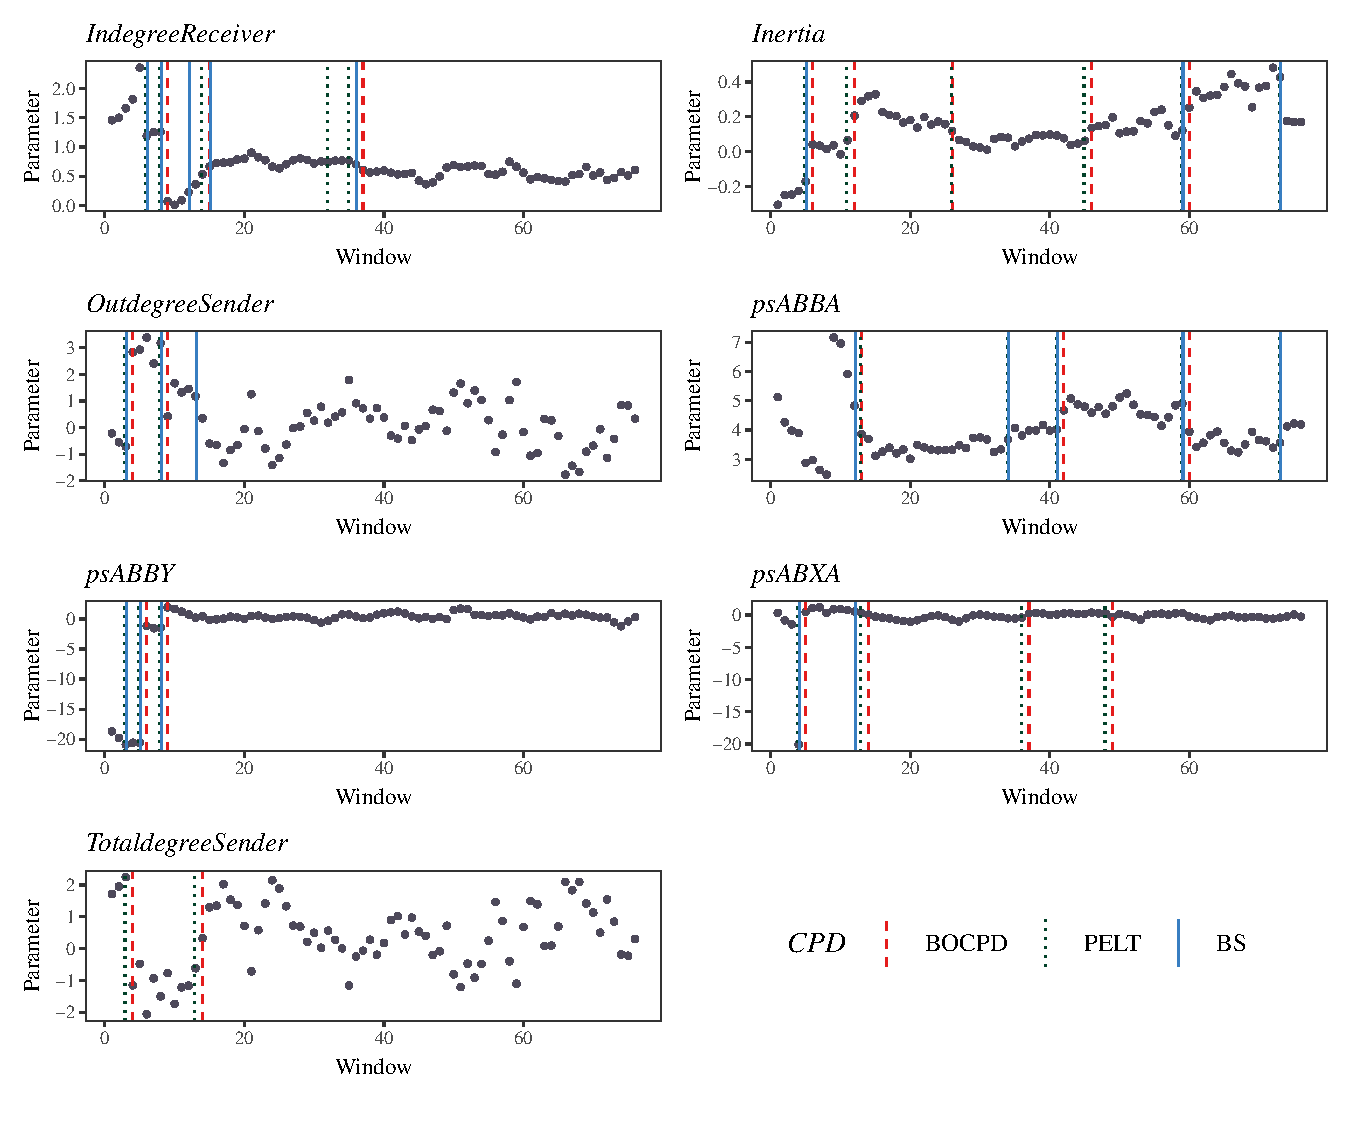
\includegraphics[width=\textwidth,height=\textheight,keepaspectratio]{Apollo_CPD_bw}
    	\caption{\fontsize{8}{10}\selectfont The plot shows the number of false positives, true positive rate, and positive predictive value of the three changepoint detection algorithms for effects without changepoint, effects with one changepoint, and effects with two changepoints.}
    	\label{Figure 6}
    \end{figure}
	
	\section{\fontsize{14}{15}\selectfont Discussion}
	
	\hspace{0.28cm} This paper proposes an approach based on the MW-REM structure to detect changepoints in social networks. Additionally, we compare the performance of three widely used changepoint detection algorithms, BOCPD, BS, and PELT, under the MW-REM structure. The proposed approach first identifies the key effects that influence social interactions in the network, and then selects an appropriate window length and overlap to segment the event history of the network. The MW-REM is then fit to the event history, and effect parameters are extracted for each fitting window of each effect. Finally, the extracted effect parameters are inputted into the changepoint detection algorithms to detect the changepoints in the network of each effect. With this approach, we can identify significant changes in the network over time and gain insights into the underlying dynamics of the network. \\
	
	The validation of our approach using synthetic data and real-life data from the Apollo 13 mission has demonstrated its effectiveness in detecting changepoints in social networks. Both the synthetic data analysis and the Apollo 13 mission analysis yielded similar conclusions: the proposed approach is capable of detecting most of the changepoints in the multivariate changepoint contexts of the social network, as all three algorithms had a high true positive rate (TPR) in the synthetic data and spotted almost all the effects' windows containing or nearing the emergency report in the Apollo 13 analysis. BOCPD performed well in precision (PPV), tending to give fewer changepoint windows but which were mostly true changepoint windows. PELT had a good TPR but a higher number of false negative cases. PELT and BS sometimes detected the changepoint window a bit earlier than the actual changepoint window in the retrieval study due to their interval merging property, where they recognize a changepoint in a certain interval. \\
	
	Overall, our approach provides a useful tool for detecting changepoints in social networks, which can be applied in various fields, such as social science, economics, and epidemiology, to identify critical changes in complex systems. Further research can explore the potential of our approach in identifying the exact time point of changepoints in the event history. As our proposed method identifies the changepoint by window periods, it infers the changepoint is within a certain time period, but not the specific time point in the event history. Shafiee Kamalabad, and Leenders et al.\cite{kamalabadWhatPointChange} suggested a Bayes factor changepoint detection method under the REM, which grids the time points of the event history and uses the support of two hypotheses from the REH to prove the existence of changepoints. By combining our method with the Bayes factor changepoint detection method, we can first identify the time period that the changepoint belongs to using our approach. Then, we can conduct the Bayes factor changepoint detection method on that period, which may provide us with the specific time point of the changepoint. This may be a promising area for further research. Additionally, future research can investigate the suitability of our approach in identifying changes in different types of networks and compare the performance of different changepoint detection algorithms under various network structures.\\
	
	
	
	
	\newpage
	
	\nocite{*} % Print all the References out, not only the citing
	\bibliographystyle{abbrv}
	\bibliography{My_Library}
	
\end{document}
